
%\Documentclass[12pt]{jreport}
\documentclass[uplatex, 12pt]{ujbook}
%%
%%  卒業論文 スタイルファイル 2026年度版
%%                       T. MATSUZAKI
%%  $Lastupdate: Tue Oct  6 15:06:48 2026 $
%%
%\begin{figure}[htpb]
% \begin{center}
%  \includegraphics[width=8cm,height=4cm,clip,keepaspectratio]{syouroku.eps}
% \end{center}
% \caption{図3.1}
% \label{fig:FIG1}
%\end{figure}

\usepackage{jgraduate20}     % jgraduate20.styを読み込む
\usepackage[dvipdfmx]{graphicx}
\usepackage[dvipdfmx]{color}
\usepackage{makeidx}          % 索引作成用
\usepackage{ascmac}	% required for `\screen' (yatex added)
\usepackage{color}
\usepackage{ulem}
\usepackage{amsmath}
\usepackage{booktabs}   % 見やすい罫線（\toprule, \midrule, \bottomrule）
\usepackage{array}      % 列幅指定（p{...}）の拡張
\usepackage{float}
%\usepackage{listings,jlisting}
\usepackage{listings}
\usepackage{url}
%\usepackage{jvlisting}
% 前設定	

\doubleside{1}                % 1:両面印刷/0:片面印刷

\title{一般家庭用Wi-FiルータのCSIを用いたWi-Fiセンシング}
\authorid{2311170016}
\author{松井　聖斗}
\university{近畿大学}                 % 大学名 (近畿大学, etc.)
\department{産業理工学部}             % 学部名 (産業理工学部, etc.)
\major{電気電子工学科}                % 学科名 (電気電子工学科, etc.)
%\date{\today}
\date{令和9年1月9日}
\year{令和八年度}
\teacherpos{教授}
\teacher{松崎　隆哲}
\coauthornum{1}                       % 共同研究者の人数 (3人まで対応)
\cfauthid{2511170001}                % 共同研究者1の学籍番号
\cfauth{川野　義了}                    % 共同研究者1の名前
\csauthid{05-9-82-004}                % 共同研究者2の学籍番号
\csauth{前田 前田}                    % 共同研究者2の名前
\ctauthid{06-9-82-001}                % 共同研究者3の学籍番号
\ctauth{飯塚 飯塚}                    % 共同研究者3の名前

\begin{document}
\maketitle                    % 表紙
\cleardoublepageskip          % 両面印刷の場合表紙の裏は白紙にします
\tableofcontents              % 目次 (↓ *のついている項目)
\listoffigures                % 図目次
\listoftables                 % 表目次
\cleardoublepageskip          % 目次と本文を分離・両面印刷の場合表紙の裏は白紙にします
\pagenumbering{arabic}        % ページ番号をアラビア数字に
\newpage

\chapter{はじめに}
\section{背景}
近年、独居高齢者世帯の増加や高齢化の進行、防犯・安全意識の高まりを背景として、屋内での状態把握、いわゆる「見守り」の重要性が高まっている。見守りを実現する主流な手段としてカメラ型・センサー型の機器があるが、室内への常時設置には次の三つの課題がある。
第一に、プライバシー侵害のリスクである。浴室や寝室などのプライベート空間への設置が困難である。
第二に、死角と環境依存のリスクである。夜間や暗所では精度が低下し、湯舟などは死角になりやすい。
第三に、設置コストのリスクである。新規機器の購入が必要であり、全室をカバーするには多数の機器を設置しなければならない。実際、介護家族を対象とした調査では、見守りサービスに約半数が関心を示す一方で、利用率は約5\%にとどまっている。\cite{sms}



\begin{figure}[htbp]
  \centering
  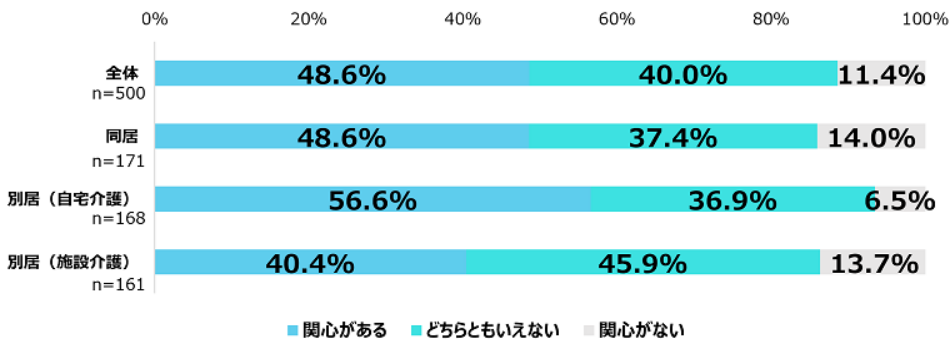
\includegraphics[width=0.8\linewidth]{mimamori_interest.png}
  \caption{被介護者と介護家族の居住形態別の見守りサービスへの関心度}
  \label{fig:result}
\end{figure}

\begin{figure}[htbp]
  \centering
  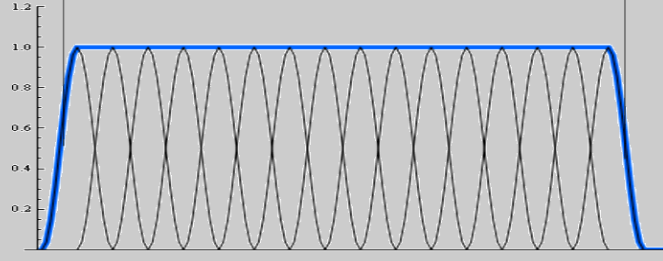
\includegraphics[width=0.8\linewidth]{mimamori_rate.png}
  \caption{見守りサービスの利用率}
  \label{fig:result}
\end{figure}

これらの課題を解決できる可能性のある技術として、Wi-FiのCSI（Channel State Information）を用いたセンシングが注目されている。
CSIは、Wi-Fi通信における伝送路特性を示すデータであり、送受信機間の空間の揺らぎを電波の振幅・位相の変化として捉えることができる。
この手法は、ほぼすべての家庭に既に設置されているWi-Fiルータを活用できるため、カメラ型に比べて導入コストの面で有利であり、映像を扱わないためプライバシーへの懸念も少ない。
本研究の目的は、家庭用Wi-Fiルータがどの程度の精度でセンシング可能かを明らかにすることである。

\section{通信インフラとしてのルータ}
家庭用Wi-Fiルータは、ほぼすべての家庭に既に設置されている通信インフラである。
また、ルータを介して家全体で通信することが可能な形で設置されることが多い。
したがって、ルータを送信機として利用できれば、センシングのために送信機を新たに購入・設置する必要がなく、すでにある通信インフラをそのままセンシングの
基盤として活用できる。
一方、専用のマイコンを送信機とする場合は、専用機器を各部屋に追加で設置し、電源を確保して運用する必要がある。
これは、導入コストを下げるという目的と相反する。
そのため、通信インフラとして利用されているルータを、そのままセンシングの送信機として利用できるかどうかは、実用化に向けて重要な論点である。
\section{先行研究}
先行研究では、Wi-FiのCSIを用いたセンシングについて、機器構成や取得方法の両面から多くの検討が行われている。
CSIの取得には、Intel5300用のCSI Tool、Atheros CSI Toolなどのツールが広く用いられている。
しかし、これらは特定のチップセットを搭載した機器を前提とし、ファームウェアやドライバの改造を必要とする。
そのため、一般の家庭にある市販ルータをそのまま利用できるとは限らない。
一方、ESP32マイコン向けのCSI取得ツールは、安価なマイコンでCSIを取得でき、改造なしに扱えることから、センシング研究に広く利用されている。


こうしたマイコンを用いた研究として、Limらは、市販ルータ(D-Link AX3000)を送信機、ESP32マイコンを受信機として使用し、見通し内及び見通し外の屋内環境で、
人物の行動を検知するためのデータセットを構築した。この研究は、家庭用Wi-Fiルータを送信機とするCSIセンシングが成立することを示しており、本研究と構成が近い。
しかし、その目的はデータセットの構築であり、ルータを用いた際のCSIセンシングの精度を、マイコン送信機の際と比較して評価することは行われていない。\cite{lim}


またZhaoらは、家庭用Wi-Fiルータを送信機、ESP32S3を受信機として使用し、パケットロスによって欠損したCSIを、BERTに着想を得た手法で復元する方法を提案した。
この研究は、ルータを送信機とした場合に、パケットの欠損が起こりうることを前提としており、ルータ送信機のCSIが、マイコン送信機の場合とは異なる性質を持つ可能性を示唆している。
しかし、パケットの到着間隔などの送信特性が、センシングの精度に与える影響までは検討されていない。\cite{zhao}

以上のように、先行研究では、ルータを送信機として利用する事例や、受信側の課題への対処が報告されているものの、家庭用ルータを送信機とした場合に、どの程度の精度でセンシングが可能かを、マイコン送信機と比較して評価した研究は十分に行われていない。特に、送信機の種類による通信間隔の違いが、検知精度にどのように影響するかは明らかになっていない。
専用機器を前提とした手法が、家庭にある機器でそのまま通用するとは限らないため、実用化に向けて、この差を把握する必要がある。

\section{本論文の構成}
本論文の構成は以下のとおりである。
第二章ではCSIを用いたWi-Fiセンシングの概要について述べる。
第三章では今回行った実験の目的と環境、手法について述べる。
第四章では送受信機の配置の違いによる評価について述べる。
第五章では複数日にわたって取得された同じ条件での測定結果に対する評価について述べる。
第六章では今回行った実験における予備評価について述べる。
第七章では今回行った実験に対する考察を述べる。
\chapter{CSIを用いたWi-Fiセンシングの概要}
\section{Wi-Fiについて}
Wi-Fiは、IEEE 802.11規格に基づく無線LANの通信方式であり、家庭や商業施設などの、様々な施設で使用されている。
ルータなどのアクセスポイントとスマートフォンやPCなどの端末が、電波を介してデータを送受信する。
使用する周波数帯には2.4GHz帯と5GHz帯があり、規格の世代によって対応する周波数帯や通信速度が異なる。

本研究で使用した機器が対応する規格は次の通りである。
AtomS3およびアンテナ付きESP32S3は、2.4GHz帯のIEEE 802.11n（Wi-Fi 4）に対応する。
ルータ（Aterm WX3000HP）は、2.4GHz帯および5GHz帯のIEEE 802.11ax（Wi-Fi 6）に対応する。
\section{OFDMについて}
Wi-Fiでは、OFDM（Orthogonal Frequency Division Multiplexing：直交周波数分割多重）と呼ばれる通信方式が用いられている。
OFDMは、送信するデータを多数の狭い帯域の搬送波（サブキャリア）に分割し、それらを同時に送信する方式である。
各サブキャリアの周波数は互いに直交するように配置されているため、周波数が重なっていても互いに干渉せず、周波数を効率よく利用できる。
送信データは、まずIQ平面上の点として表される複素数 a+jb（jは虚数単位）に変換される。
たとえば4値の位相変調では、2ビットの組（00, 01, 10, 11）がIQ平面上の4点に対応する。この複素数を各サブキャリアに割り当て、64本のサブキャリアを重ね合わせることでOFDM信号が構成される。\cite{OFDM}
OFDMは、周波数ごとに伝送路の特性を扱えるという特徴がある。この特徴により、周波数ごとの伝送路の状態を表す情報（次節のCSI）を、サブキャリア単位で得ることができる。
Wi-Fi電波は、空間を伝搬する間に壁や家具、人体などで反射・散乱・減衰し、複数の経路を経由して受信機に届く。
そのため、受信信号は送信信号に比べて振幅が減衰し、位相がずれる。CSIは、この送信信号から受信信号への変化を、サブキャリアごとに表したものである。

\section{CSIについて}
\subsection{CSIの仕組み}
CSI（Channel State Information：チャネル状態情報）とは、Wi-Fi通信における伝送路特性を示すデータである。
送信された信号SIは複素数の行列として取得され、その要素 $h_{ij}$ は次のように実部 $a_{ij}$ と虚部 $b_{ij}$ で表される。
\begin{equation}
h_{ij} = a_{ij} + j·b_{ij}
\end{equation}
この複素数から、振幅の減衰度と位相のずれを次式で計算できる。
\begin{align}
振幅：r &= \sqrt{a_{ij}^2 + b_{ij}^2}\\
位相：\theta &= \tan^{-1}\left(\frac{b_{ij}}{a_{ij}}\right)
\end{align}

本研究で用いるESP32では、受信したパケットのHT-LTFからCSIを取得する。タイムスタンプ、パケット番号、および64組のサブキャリアの虚部と実部が、この順に出力される。
\subsection{CSIのセンシングへの利用}
伝送路上の物体や人が動くと、反射・散乱の状態が変化し、CSIの振幅と位相が変化する。
この変化を観測することで、送受信機間の空間で生じた動きを推定できる。これがCSIを用いたWi-Fiセンシングの原理である。
この手法は、既存のWi-Fi通信の電波をそのまま利用するため、カメラ型のセンシングとは異なり映像を取得する必要がない。
また、すでに設置されているWi-Fi機器を活用できる。このため、導入コストの面で有利であり、プライバシーへの懸念も少ない。
本研究では、CSIの変化を引き起こす要因としてNCフライス盤のドリルの回転を用い、取得したCSIの振幅データを機械学習で分類することで、センシングの精度を評価する。


\chapter{各送受信機のCSI取得方法}
本章では、本研究で用いる送信機と受信機について、CSIをどのように取得するかを述べる。
送信機にはルータ、AtomS3、アンテナ付きESP32S3の3種類を用い、受信機にはAtomS3とアンテナ付きESP32S3の2種類を用いた。

\section{CSI取得の全体像}
CSIは、受信機が送信機からのパケットを受信した際に、そのパケットから取得される。
したがって、CSIを取得するには、送信機が継続的にパケットを送信し、受信機がそれを受信する必要がある。
送信機の種類によって、パケットを送信させる方法が異なる。

受信機（AtomS3、アンテナ付きESP32S3）では、Espressif Systemsが提供するESP32用のCSI取得ツールesp-csi\cite{espcsi}を用いてCSIを取得した。
受信したパケットのHT-LTFからCSIを取得し、タイムスタンプ、パケット番号、および64組のサブキャリアの虚部と実部が、この順に出力される。

\section{各送信機のCSI取得}
AtomS3およびアンテナ付きESP32S3を送信機とする場合は、送信機側のマイコン自身が一定の間隔でパケットを送信し、受信機がそのパケットからCSIを取得した。

それに対しルータは、CSIを取得するための専用機能や、パケットを任意の間隔で送信させる機能を持たない。
そこで本研究では、ルータ送信機の場合、次の方法でCSIを取得した。
受信機（ESP32系マイコン）からルータに対してPingを継続的に送信し、ルータが返すPing replyを受信機が受け取る。
受信機は、このPing replyのパケットからCSIを取得する。
この方法では、ルータのファームウェアの書き換えなどの改造を必要とせず、純正のままのルータを送信機として利用できる。
通信インフラとして稼働しているルータを、そのままセンシングの送信機として利用できる点が、この方法の利点である。
ただし、Ping replyの送信間隔は、ルータ側の処理や通信状況に左右される。
そのため、マイコン送信機に比べてパケットの到着間隔は不規則になることがある。

\chapter{実験：共通条件}
\section{実験目的}
本研究の実験の目的は、人間の動きと比べ動きが常に一定であるNCフライス盤のドリルの回転数を識別対象とし、送信機にルータとマイコンを用いた場合の分類精度を比較することにより、
家庭用Wi-Fiルータがどの程度の精度でセンシング可能かを明らかにすることである。
さらに予備評価として、次の3点に対応した追加実験も行った。

\begin{itemize}
  \item チャネルの違いによって精度に差が出るのか
  \item 取得したデータは、その条件でしか使えないのか
  \item 環境や測定対象が変わっても使えるか
\end{itemize}
上記に対応して行った実験を表3.1に示す。

\begin{table}[htbp]
  \centering
  \caption{実験の一覧}
  \label{tab:experiments}
  \begin{tabular}{l p{6.5cm} p{4.5cm}}
    \toprule
    実験 & 目的 & 変更した条件 \\
    \midrule
    実験1 基礎評価 & 送信機・受信機・距離条件ごとの精度を比較 & 送受信機の組み合わせ、距離条件 \\
    実験2 チャネル入れ替え & チャネルによる影響の切り分け & チャネル（ch1とch11） \\
    実験3 複数日測定 & 日による環境差の影響の確認 & 測定日（3日間） \\
    実験4 別部屋・別機械 & 環境・機械の違いへの汎化性の確認 & 部屋、機械、回転数 \\
    \bottomrule
  \end{tabular}
\end{table}

\clearpage
\section{使用デバイス}
実験には、送信機としてルータとマイコン、受信機としてマイコンを用いた。使用したデバイスの仕様を表3.2に示す。
ルータには、改造を行っていない市販品をそのまま用いた。
ESP32系マイコンは、CSI取得ツールesp-csiを用いて、受信機としてCSIを取得した。
また、回転体としてNCフライス盤のドリルを用いた。
追加実験（実験4）では、別の機械としてHOZAN K-21（3段ベルト変速で2100、4500、6200rpm）を用いた。

\begin{table}[htbp]
  \centering
  \caption{使用デバイスの仕様}
  \label{tab:devices}
  \small
  \begin{tabular}{l l l l l l}
    \toprule
    デバイス & 用途 & マイコン & フラッシュ & 無線機能 \\
    \midrule
    AtomS3 & 送信機・受信機 & ESP32-S3 & 8\,MB & 2.4\,GHz Wi-Fi 4  \\
    アンテナ付きESP32S3 & 送信機・受信機 & ESP32-S3 & 8\,MB & 2.4\,GHz Wi-Fi 4  \\
    Aterm WX3000HP & 送信機 & --- & --- & 2.4/5\,GHz Wi-Fi 6  \\
    \bottomrule
  \end{tabular}
\end{table}

\begin{figure}[htbp]
  \centering
  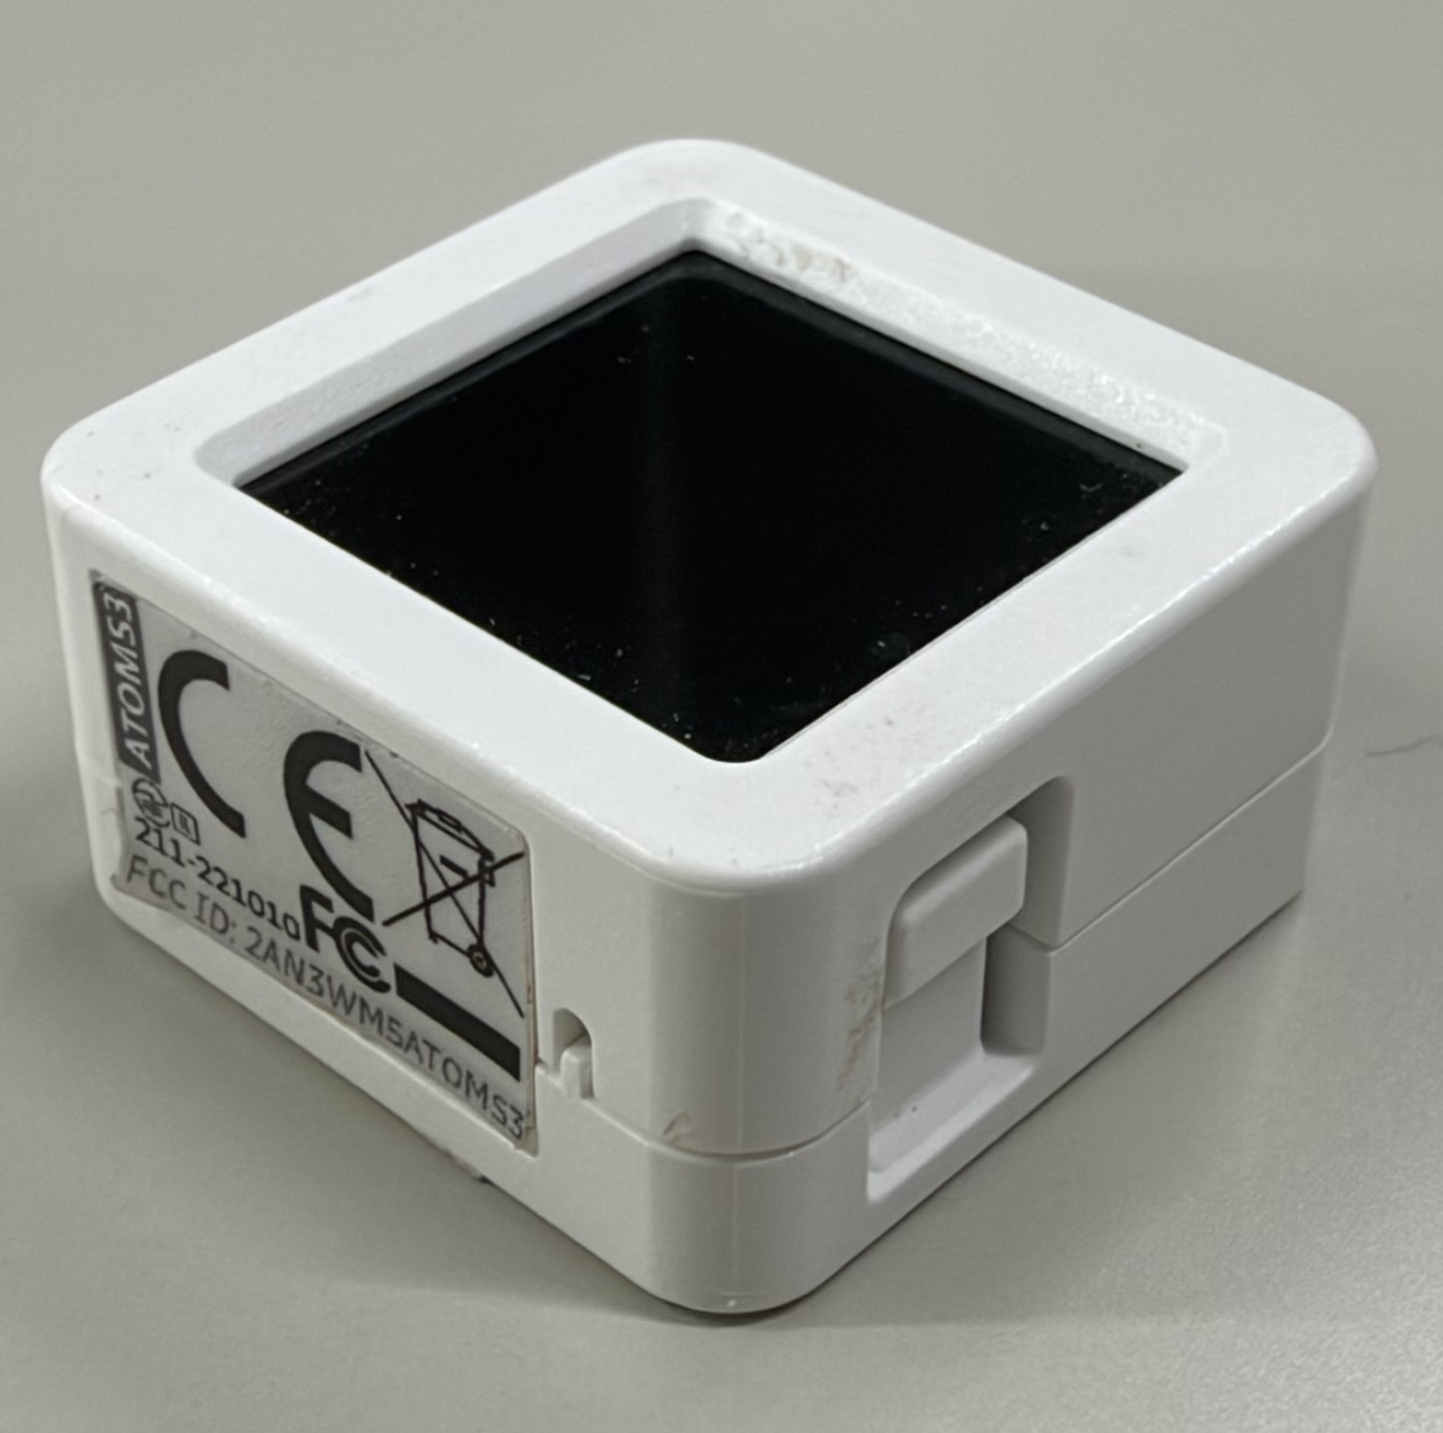
\includegraphics[width=0.5\linewidth]{AtomS3.png}
  \caption{AtomS3}
  \label{fig:result}
\end{figure}

\begin{figure}[htbp]
  \centering
  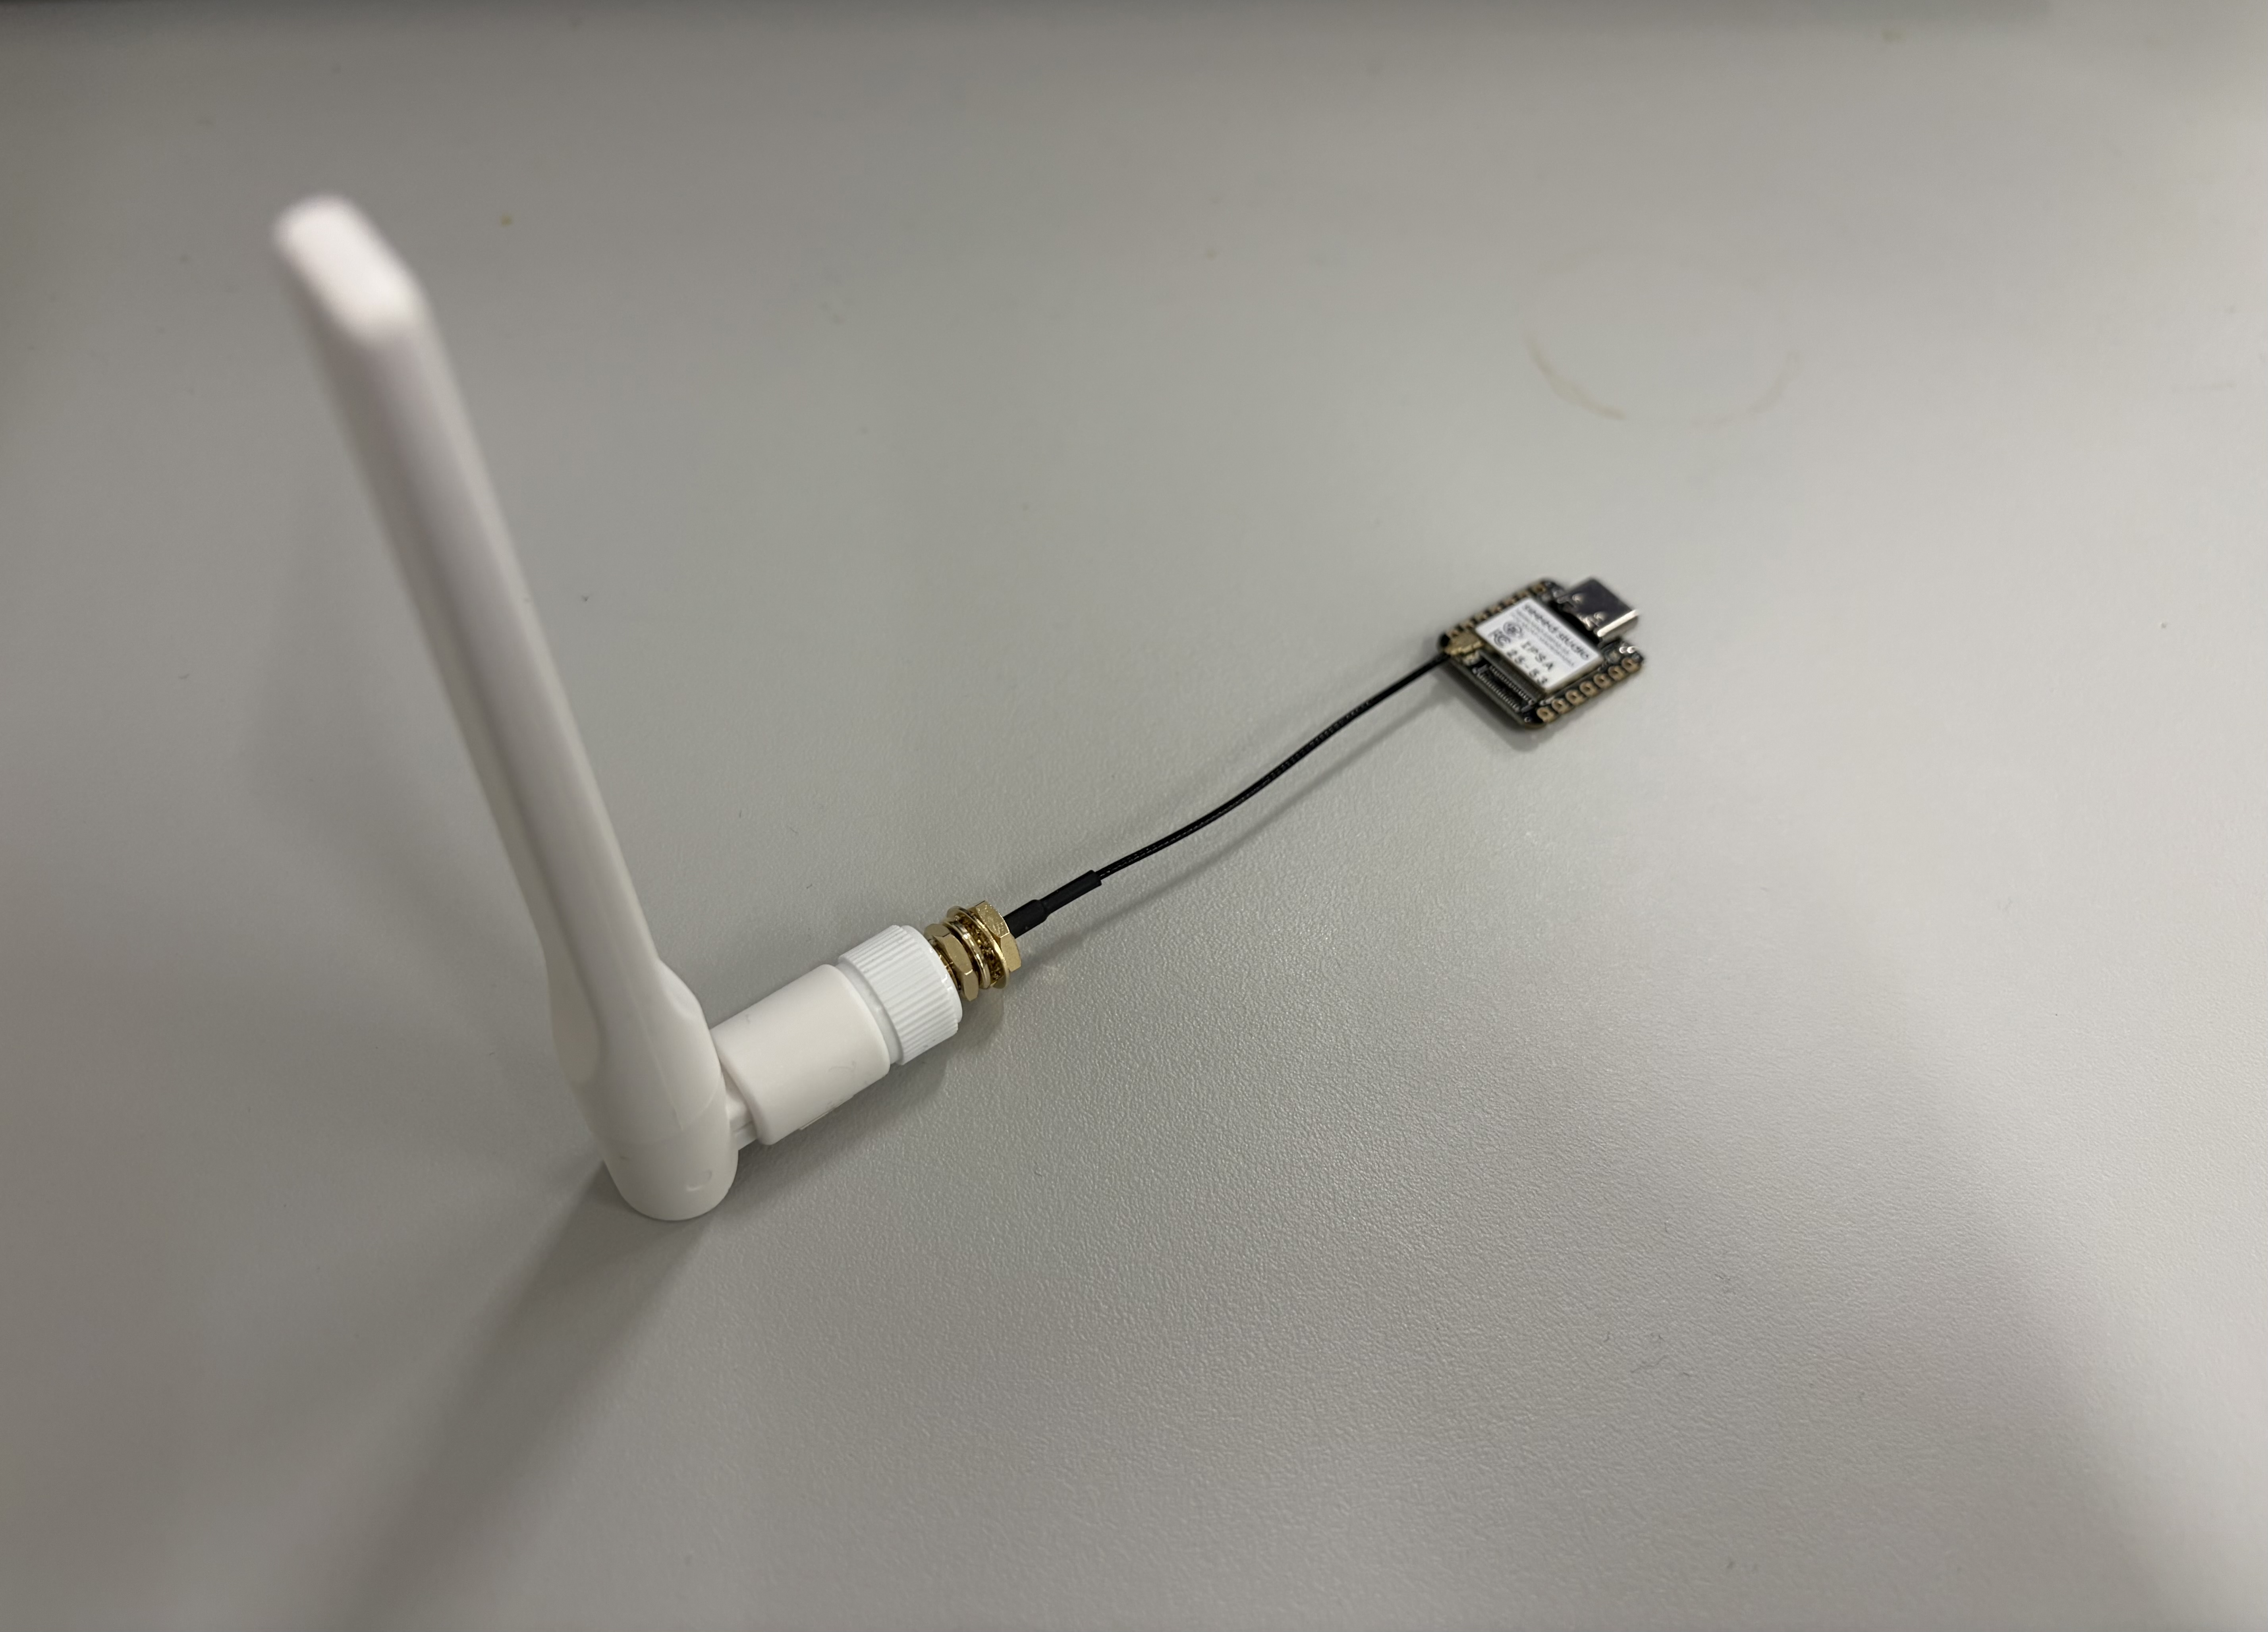
\includegraphics[width=0.5\linewidth]{esp32s3.png}
  \caption{esp32s3}
  \label{fig:result}
\end{figure}

\begin{figure}[htbp]
  \centering
  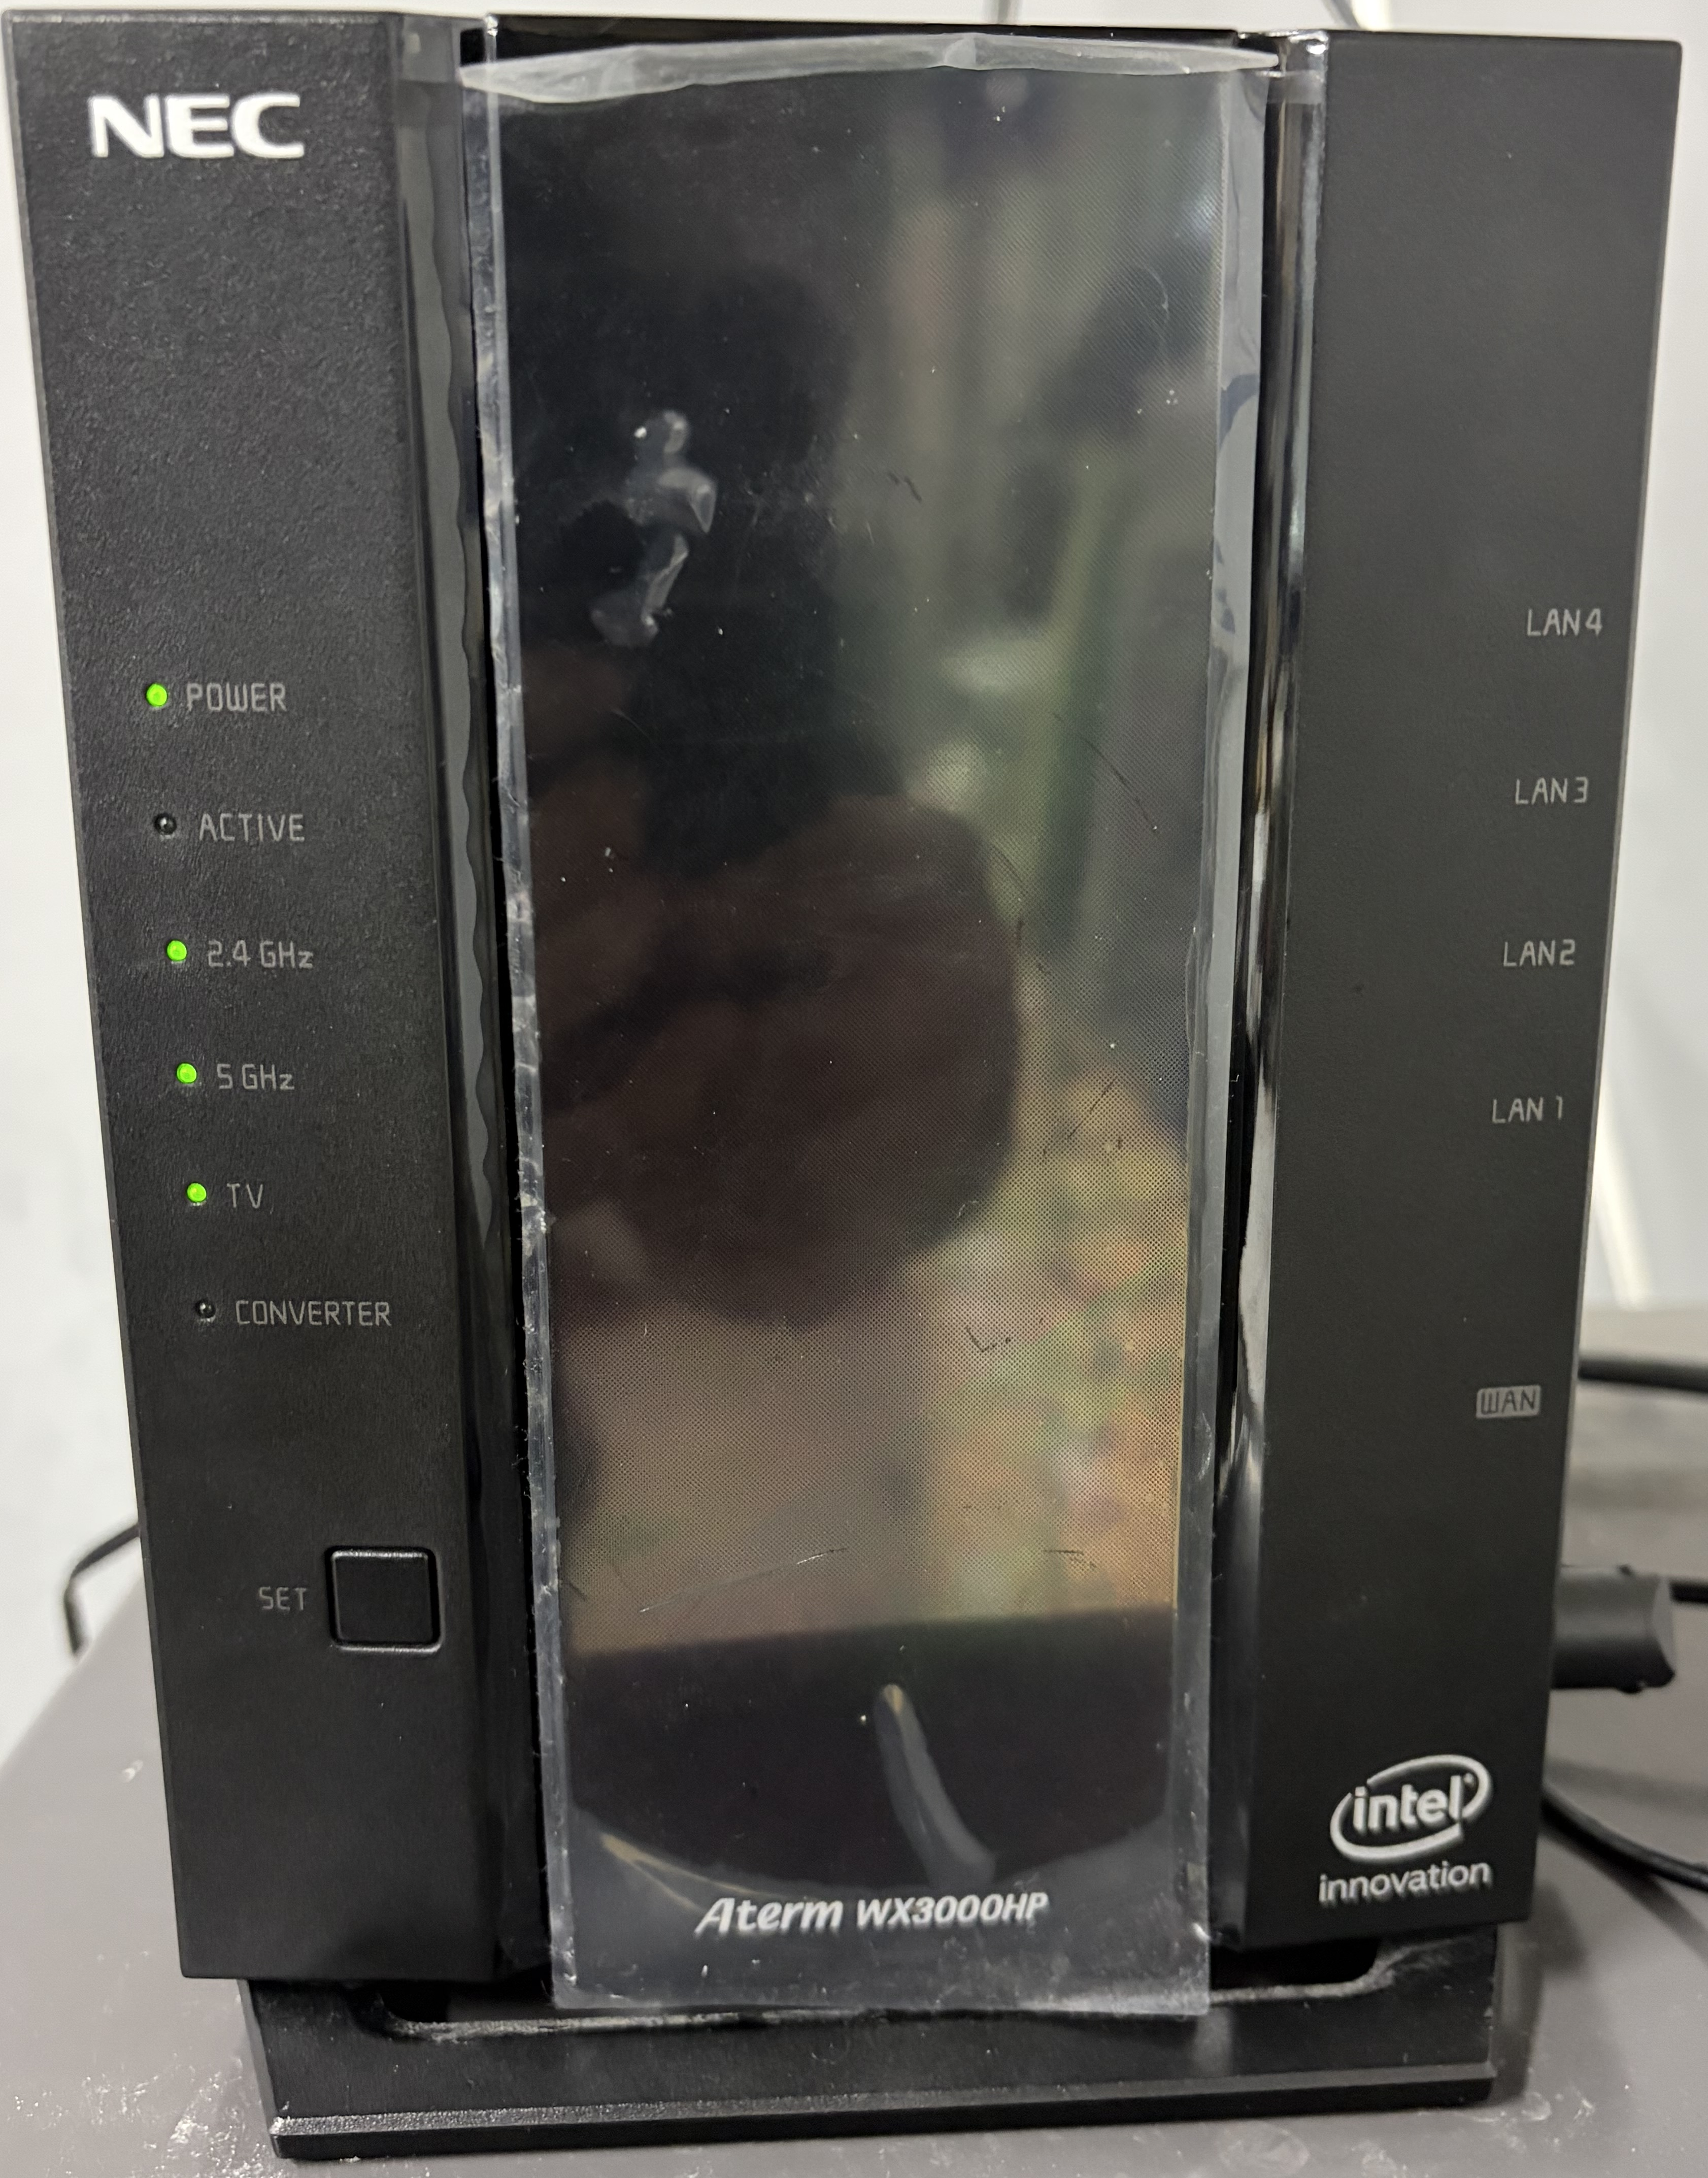
\includegraphics[width=0.5\linewidth]{router.png}
  \caption{使用したルータ(Aterm WX3000HP)}
  \label{fig:result}
\end{figure}

\begin{figure}[htbp]
  \centering
  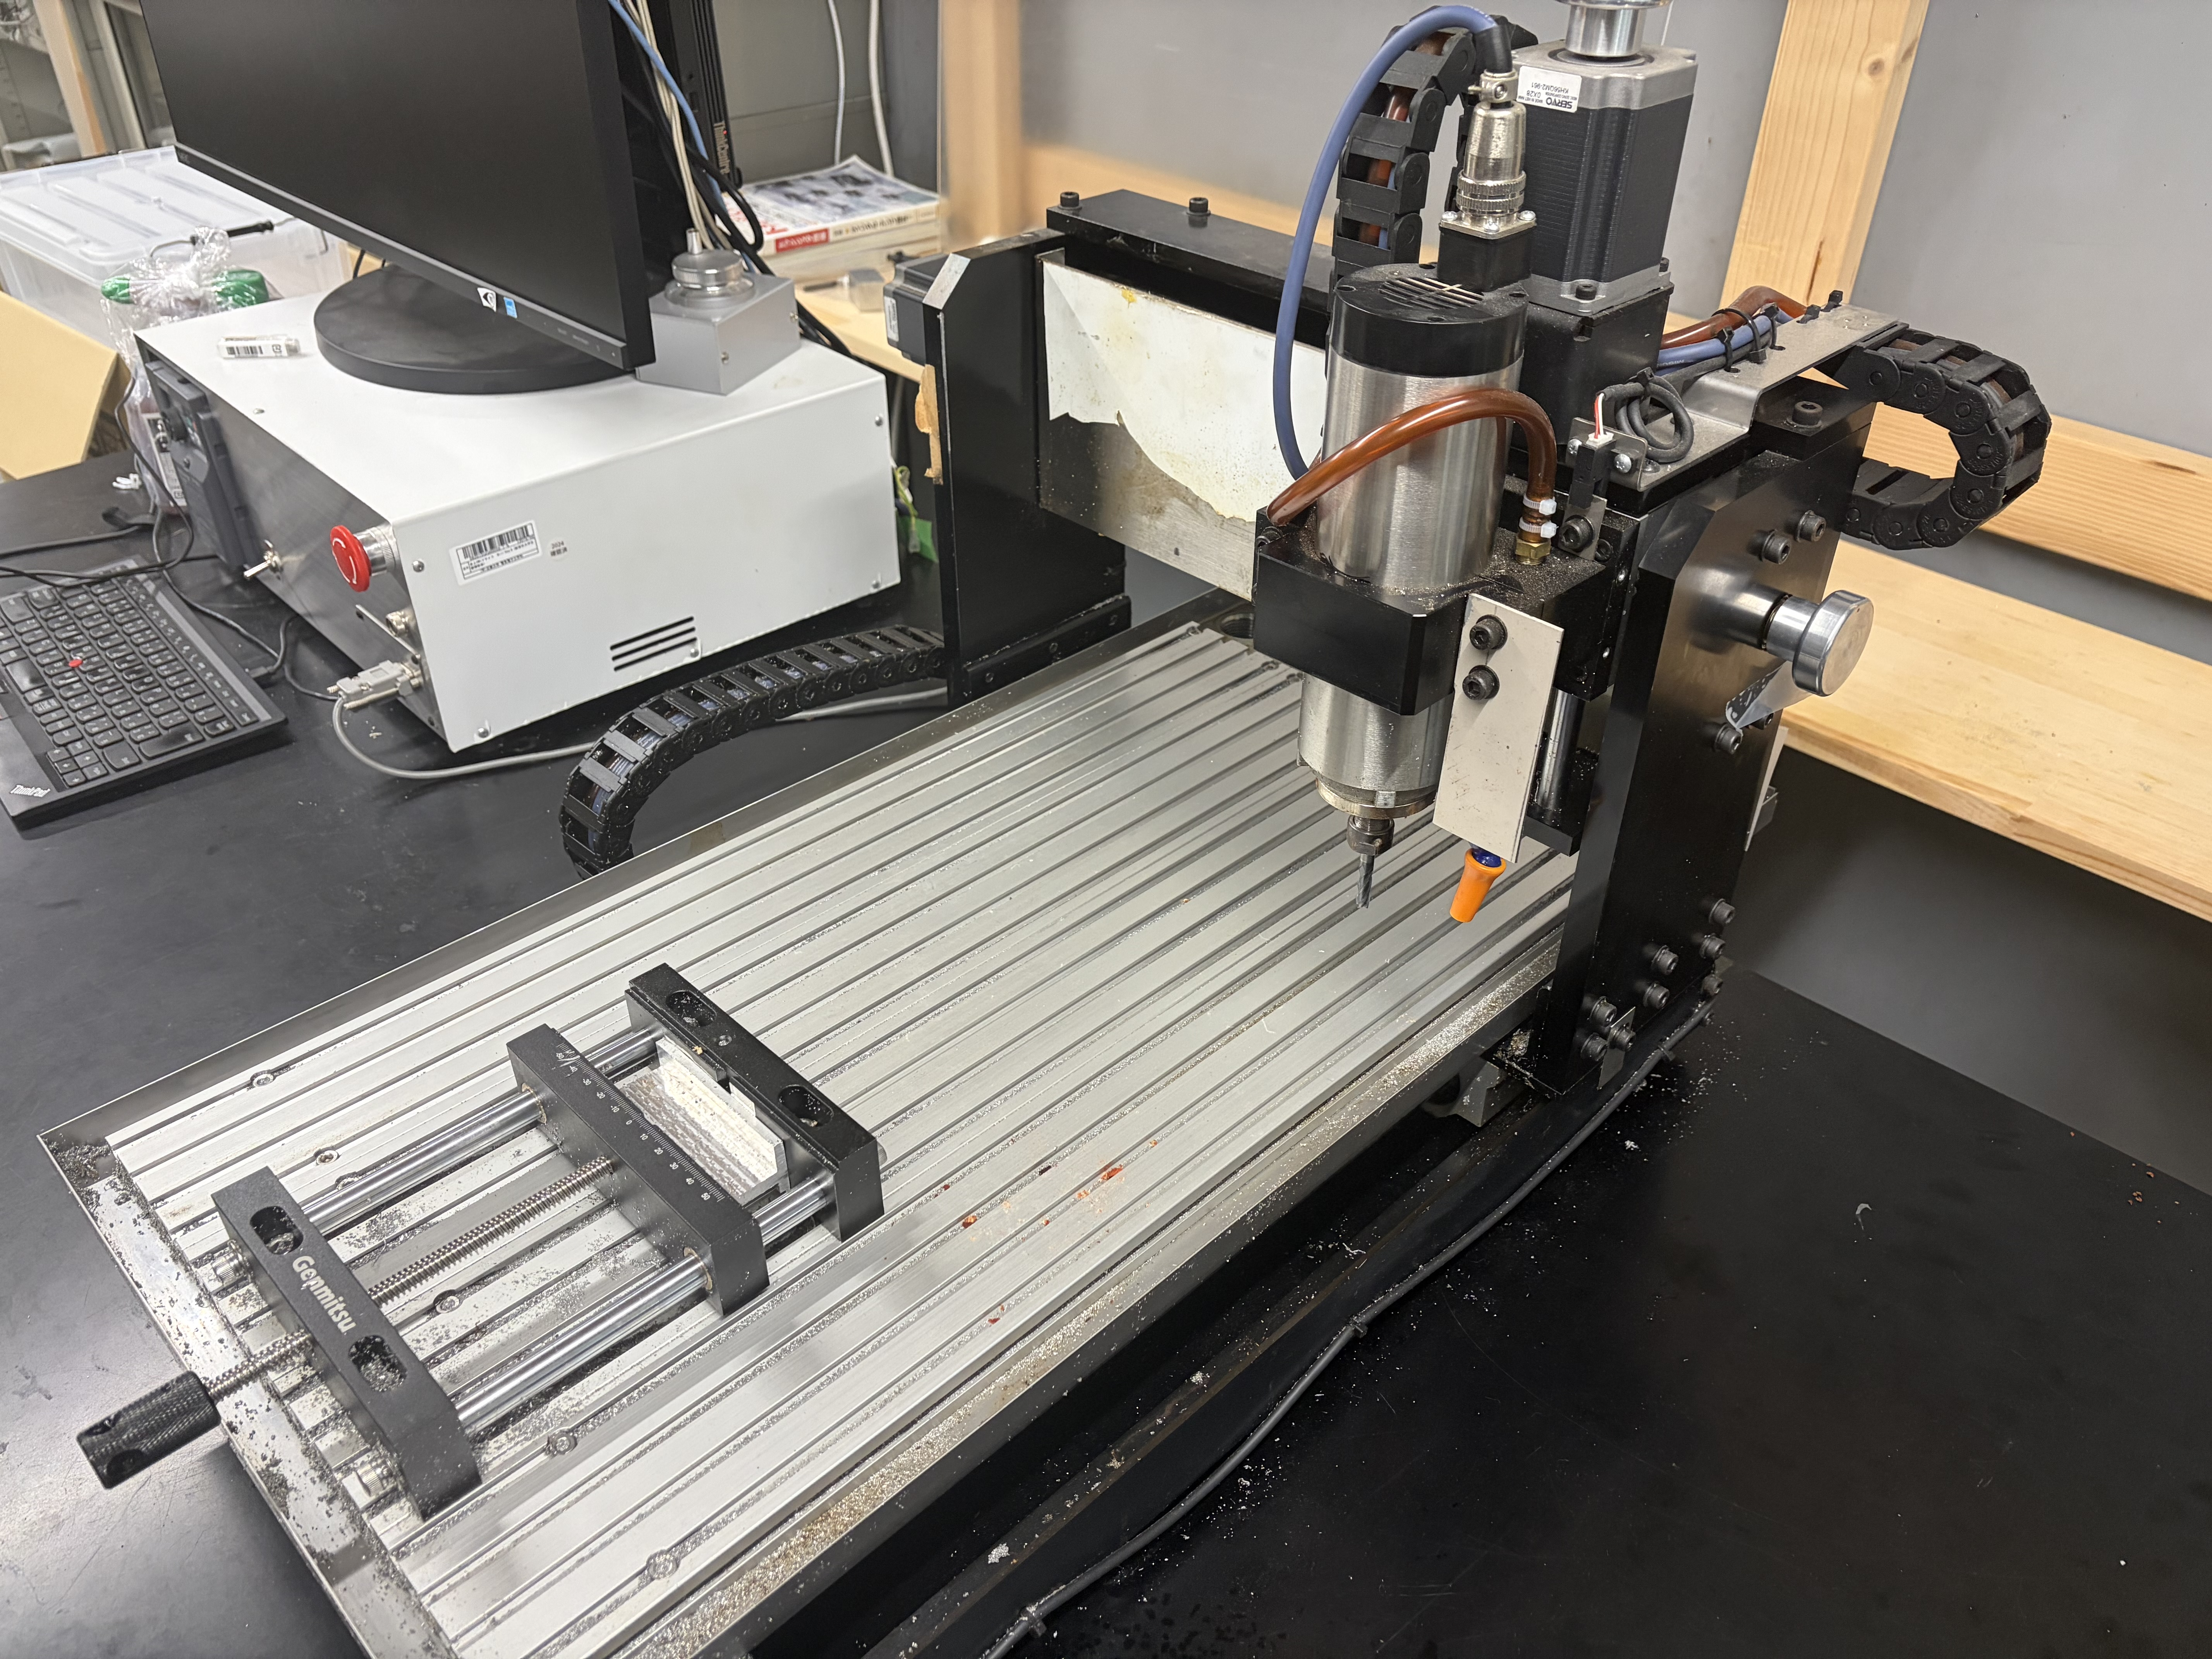
\includegraphics[width=0.8\linewidth]{NC.png}
  \caption{NCフライス盤}
  \label{fig:result}
\end{figure}

\newpage
\section{実験環境}
\subsection{実験室}
実験1〜3は、2214ものづくり工房で行った。部屋の大きさは4.3m×8.7mである。
実験4は、ものづくり工房より広い部屋で行った。
\subsection{送受信機の配置}
送受信機は、NCフライス盤を結ぶ直線上に、送受信機間に直接的な障害物がないように配置した。
距離条件は次の3種類である。
\begin{table}[htbp]
  \centering
  \caption{距離条件と配置}
  \label{tab:layout}
  \begin{tabular}{l c c c c}
    \toprule
    条件 & 送信機の距離 & 受信機の距離 & 送信機の高さ & 受信機の高さ \\
    \midrule
    near-near & 0.5\,m & 0.3\,m & 0.69\,m & 0.83\,m \\
    far-near  & 5.9\,m & 0.3\,m & 1.1\,m  & 0.83\,m \\
    far-far   & 5.9\,m & 1.0\,m & 1.1\,m  & 0.80\,m \\
    \bottomrule
  \end{tabular}
\end{table}
なお、各距離は、NCフライス盤からの距離である。
\section{実験条件}
% ===== 以下、仮の下書き（2026/11/23）。【要確認】の箇所は事実関係を確認すること =====
\subsection{識別対象}
実験1〜3では、NCフライス盤のドリルを0、3000、6000、9000\,rpmの4段階で回転させ、この4つの回転数を分類のクラスとした。
0\,rpmは、ドリルを停止させた状態である。
ドリルの回転は、人間の動作と異なり、同じ回転数であれば常に同じ周期で同じ動きを繰り返す。
そのため、識別対象の側のばらつきを抑えたうえで、送信機や配置の違いによる精度の差を比較できる。

\subsection{使用チャネル}
送受信は2.4\,GHz帯で行った。
実験1および実験3では、ルータを送信機とする場合はch1、マイコンを送信機とする場合はch11を使用した。
実験2では、このチャネルを入れ替えた（第6章）。

\subsection{パケットの送信}
マイコン（AtomS3、アンテナ付きESP32S3）を送信機とする場合は、送信機のマイコンが一定の間隔でパケットを送信した。
% 【要確認】マイコン送信機の送信間隔の設定値（実測の受信レートはAtomS3で約124\,Hz、ESP32S3で約97\,Hz）
ルータを送信機とする場合は、第3章で述べたように、受信機からルータのゲートウェイアドレスに対してPingを10\,ms間隔（100\,Hz）で送信し続け、
ルータから返ってくるPing replyからCSIを取得した。

\subsection{測定手順}
測定は次の手順で行った。
\begin{enumerate}
  \item 送信機と受信機を表\ref{tab:layout}の距離条件のとおりに配置する。
  \item 受信機をUSBシリアル（921600\,bps）でPCに接続し、受信機が出力するCSIをPython のプログラムで読み取る。
  \item ドリルを測定する回転数に設定し、回転が安定してから測定を開始する。
  \item 一定数のパケットのCSIを1つのファイルとして保存し、これを繰り返す。
  \item 1つの回転数で所定のファイル数がそろったら、回転数を変えて3.〜4.を繰り返す。
\end{enumerate}
1ファイルあたりのパケット数は、マイコン送信機では300パケット、ルータ送信機では500パケットとした。
各回転数につき500ファイルを取得し、1つの測定条件あたり4クラス計2000ファイルとした。
% 【要確認】測定中の人の在室・退出、測定開始直後のファイルを捨てたかどうか（data_capture_and_convert.ipynb では先頭5ファイルを破棄している）
% 【要確認】ルータ送信を500パケットにした理由（Ping replyの欠損を見込んで多めにした、など）

\section{評価方法}
本研究では、XGBoostという学習器を用いて、機械学習による分類の精度を評価した。

\subsection{前処理}
受信機から出力される1パケット分のCSIは、64本のサブキャリアそれぞれの虚部$b$と実部$a$からなる。
各サブキャリアについて、式(2.2)により振幅$r=\sqrt{a^2+b^2}$を計算した。
1ファイルを1つのサンプルとし、ファイル内の全パケット・全サブキャリアの振幅を1次元に並べたものを特徴量とした。
各サンプルには、測定したときの回転数を正解ラベル（0〜3）として与えた。
% 【要確認】特徴量を「全パケット連結」にするか「振幅の時間平均（57本）」にするか。
%  use_program/machine_learning.py は全パケット連結、技術メモ・再現解析は時間平均を主に使っている

\subsection{データの分割}
各測定条件のデータを、クラスの比率を保ったまま（層化抽出）、学習用80\,\%とテスト用20\,\%に分割した。
さらに、学習用のデータを同様に80\,\%と20\,\%に分け、後者を検証用データとして学習の早期終了の判定に用いた。
テスト用のデータは学習には一切使わず、最終的な精度の評価にのみ用いた。
% 【要確認】乱数シードを固定したか、何回繰り返して平均したか

\subsection{学習の設定}
XGBoostの設定を表\ref{tab:xgb}に示す。
多クラス分類として学習し、検証用データの損失が10ラウンド続けて改善しなければ学習を打ち切った。
\begin{table}[htbp]
  \centering
  \caption{XGBoostの設定}
  \label{tab:xgb}
  \begin{tabular}{l l}
    \toprule
    項目 & 設定値 \\
    \midrule
    目的関数 & multi:softmax（多クラス分類） \\
    クラス数 & 4 \\
    評価指標（学習時） & mlogloss（多クラス対数損失） \\
    最大ラウンド数 & 100 \\
    早期終了 & 10ラウンド \\
    その他 & 既定値 \\
    \bottomrule
  \end{tabular}
\end{table}

\subsection{評価指標}
テスト用データに対する正解率（Accuracy）とマクロ平均F1値を評価指標とした。
正解率は、テストデータ全体のうち正しく分類されたサンプルの割合である。
\begin{equation}
  \mathrm{Accuracy} = \frac{\text{正しく分類されたサンプル数}}{\text{テストサンプル数}}
\end{equation}
F1値は、クラス$k$の適合率$P_k$と再現率$R_k$の調和平均であり、マクロ平均F1値はこれを全クラスで平均したものである。
\begin{equation}
  F1_k = \frac{2P_kR_k}{P_k+R_k},\qquad
  \mathrm{Macro\mbox{-}F1} = \frac{1}{K}\sum_{k=1}^{K} F1_k
\end{equation}
ここで$K$はクラス数（本研究では4）である。
また、どの回転数をどの回転数と取り違えたかを確認するため、混同行列も作成した。

\subsection{XGBoostの理論}
XGBoost（eXtreme Gradient Boosting）は、決定木を弱学習器とする勾配ブースティングの手法である\cite{xgboost}。
勾配ブースティングでは、決定木を1本ずつ順に追加し、それまでの木の予測で残った誤差を、新しい木が補正するように学習する。
$t$本目の木を追加した後のサンプル$i$に対する予測値$\hat{y}_i^{(t)}$は次式で表される。
\begin{equation}
  \hat{y}_i^{(t)} = \hat{y}_i^{(t-1)} + f_t(\boldsymbol{x}_i)
\end{equation}
ここで$f_t$は$t$本目の決定木、$\boldsymbol{x}_i$はサンプル$i$の特徴量である。
XGBoostは、損失関数$l$に木の複雑さに対する正則化項$\Omega$を加えた次の目的関数を最小化するように、$f_t$を決める。
\begin{equation}
  \mathcal{L}^{(t)} = \sum_{i} l\left(y_i,\ \hat{y}_i^{(t-1)} + f_t(\boldsymbol{x}_i)\right) + \Omega(f_t),\qquad
  \Omega(f) = \gamma T + \frac{1}{2}\lambda \sum_{j=1}^{T} w_j^2
\end{equation}
$T$は木の葉の数、$w_j$は葉$j$の出力値、$\gamma$と$\lambda$は正則化の強さを決める係数である。
XGBoostは、損失関数を2次までテイラー展開して近似することで、各葉の最適な出力値と、分岐による目的関数の改善量を解析的に求める。
これにより、学習が高速であり、正則化によって過学習を抑えられる。

多クラス分類では、クラスごとに木を学習し、各クラスの出力をソフトマックス関数で確率に変換する。
本研究で用いたmulti:softmaxは、確率が最も大きいクラスを予測結果として出力する。
本研究の特徴量は次元数が大きい（1サンプルあたり数万次元）が、決定木は分類に有効な特徴量を選んで分岐するため、このような高次元のデータにも適用しやすい。
% 【要確認】次元数の記述は特徴量を全パケット連結にした場合（300パケット×64本=19200など）

\chapter{実験1：送信機・受信機・距離条件による精度比較}
\section{目的}
送信機の種類（ルータ、AtomS3、アンテナ付きESP32S3）、受信機の種類、距離条件によって、回転数の分類精度がどのように変わるかを明らかにする。

\section{実験条件}
送受信機の組み合わせ（6通り）と距離条件（3通り）で測定した。条件の詳細は第四章に示した通りである。
% 【要確認】data フォルダにある組み合わせは R→A, A→A, E→E, A→E, E→A の5通り。「6通り」でよいか
測定した条件と測定日を表\ref{tab:exp1}に示す。
ルータ送信機の条件は、ルータ→AtomS3の各距離条件を3回ずつ測定した。
ここでは、そのうち1回目の測定（6月）を実験1の結果として用い、2回目・3回目は実験3で用いる。
% 【要確認】実験1でどの日のルータデータを使うか（1回目のみ／3回の平均など）
いずれの条件でも、ルータ送信機はch1、マイコン送信機はch11を使用した。

\begin{table}[htbp]
  \centering
  \caption{実験1の測定条件と測定日}
  \label{tab:exp1}
  \begin{tabular}{l l c c c}
    \toprule
    送信機 & 受信機 & near-near & far-near & far-far \\
    \midrule
    ルータ & AtomS3 & 6/18 & 6/22 & 6/29 \\
    AtomS3 & AtomS3 & 6/30 & 6/30 & 7/3 \\
    アンテナ付きESP32S3 & アンテナ付きESP32S3 & 7/6 & 7/6 & 7/7 \\
    AtomS3 & アンテナ付きESP32S3 & 7/14 & 7/16 & 7/20 \\
    アンテナ付きESP32S3 & AtomS3 & 7/21 & 7/21 & 7/27 \\
    \bottomrule
  \end{tabular}
\end{table}

\section{実験方法}
表\ref{tab:exp1}の15条件それぞれについて、第4章の手順で0、3000、6000、9000\,rpmのCSIを各500ファイル取得した。
条件ごとに、第4.5節の方法で学習用・検証用・テスト用にデータを分割し、XGBoostで4クラスの分類を行った。
学習とテストには同じ条件（同じ日・同じ配置）のデータを用い、条件どうしでデータを混ぜることはしない。
得られた正解率とマクロ平均F1値を、次の3つの観点で比較した。
\begin{itemize}
  \item 送信機の違い：受信機と距離条件をそろえ、ルータ、AtomS3、アンテナ付きESP32S3を比べる。
  \item 受信機の違い：送信機と距離条件をそろえ、AtomS3とアンテナ付きESP32S3を比べる。
  \item 距離条件の違い：送受信機をそろえ、near-near、far-near、far-farを比べる。
\end{itemize}
また、ルータ送信機とマイコン送信機ではパケットの到着間隔が異なるため、各条件の受信レート（1秒あたりに受信できたパケット数）と、パケット到着間隔のばらつきも求め、精度との関係を調べた。
% 【要確認】受信レートの比較を実験1に入れるか（第3章の「到着間隔が不規則」の話とつながる）

\chapter{実験2：チャネルを入れ替えた検証}
\section{目的}
実験1では、ルータ送信機はch1、マイコン送信機はch11を使用していた。
そのため、送信機の違いによる精度差に、チャネルの違いが混ざっている可能性がある。
チャネルを入れ替えて、送信機の違いによる影響だけを取り出す。

\section{実験条件}
ルータをch11、マイコンをch1に切り替え、ほかは実験1と同じ条件で測定した。
距離条件は、送信機を遠く、受信機を近くに置くfar-nearに固定した。
測定した条件と測定日を表\ref{tab:exp2}に示す。
比較のため、元のチャネル（ルータch1、AtomS3 ch11）でも改めて測定した。

\begin{table}[htbp]
  \centering
  \caption{実験2の測定条件と測定日（距離条件はすべてfar-near）}
  \label{tab:exp2}
  \begin{tabular}{l l c l}
    \toprule
    送信機 & 受信機 & チャネル & 測定日 \\
    \midrule
    ルータ & AtomS3 & ch11 & 9/7, 9/8, 9/10, 10/1 \\
    AtomS3 & AtomS3 & ch1 & 9/14, 9/17 \\
    アンテナ付きESP32S3 & アンテナ付きESP32S3 & ch1 & 9/24 \\
    アンテナ付きESP32S3 & AtomS3 & ch1 & 9/28 \\
    \midrule
    ルータ & AtomS3 & ch1（元のチャネル） & 10/4 \\
    AtomS3 & AtomS3 & ch11（元のチャネル） & 10/28 \\
    \bottomrule
  \end{tabular}
\end{table}

\section{実験方法}
各条件について、実験1と同じく0、3000、6000、9000\,rpmのCSIを各500ファイル取得し、同じ条件内で学習・テストを行った。
分割の方法とXGBoostの設定は実験1と同じである。
次の2点を比較することで、精度の差がチャネルによるものか、送信機によるものかを判断した。
\begin{itemize}
  \item 同じ送信機で、チャネルを入れ替える前（実験1）と後（実験2）の精度を比べる。
        チャネルの影響が大きければ、入れ替えによって精度が変わる。
  \item 同じチャネルで、ルータ送信機とマイコン送信機の精度を比べる。
        送信機の影響が大きければ、チャネルをそろえても精度の差が残る。
\end{itemize}

\chapter{実験3：複数日データの評価}
\section{目的}
同一日に取得したデータで評価した精度が、日による環境の違いに依存していないかを確認する。

\section{実験条件}
3日にわたり、1日あたり0、3000、6000、9000\,rpmを1回ずつ測定した。
送受信機はルータ→AtomS3とし、3つの距離条件それぞれについて、別の日に3回測定した（表\ref{tab:exp3}）。
チャネルはch1である。
% 【要確認】実験3として使うデータがこの9条件でよいか。far-near は 9/7〜10/4 にも測定がある（ch11を含む）
\begin{table}[htbp]
  \centering
  \caption{実験3の測定日（ルータ→AtomS3、ch1）}
  \label{tab:exp3}
  \begin{tabular}{l c c c}
    \toprule
    距離条件 & 1日目 & 2日目 & 3日目 \\
    \midrule
    near-near & 6/18 & 7/9 & 8/3 \\
    far-near  & 6/22 & 7/10 & 8/4 \\
    far-far   & 6/29 & 7/11 & 8/6 \\
    \bottomrule
  \end{tabular}
\end{table}

\section{実験方法}
実験1では、同じ日に取得したデータを学習用とテスト用に分けて評価した。
この方法では、学習とテストのデータが同じ日の同じ環境で取得されているため、日による環境の違いが精度に含まれない。
そこで、学習に使う日とテストに使う日を分け、次の2通りの方法で評価した。
\begin{itemize}
  \item 日ごとの組み合わせ：ある1日のデータすべてで学習し、同じ距離条件の別の1日のデータでテストする。3日から2日を選ぶ順列6通りすべてについて行う。
  \item leave-one-day-out：同じ距離条件の3日のうち2日のデータで学習し、残りの1日でテストする。テストする日を入れ替えて3回行う。
\end{itemize}
XGBoostの設定は実験1と同じとし、検証用データは学習に使う日のデータから20\,\%を取り出した。
同じ日の中で評価した精度（実験1と同じ方法）と、日をまたいで評価した精度を比較し、精度が日によらず保たれるかを確認した。
評価が4クラスであるため、ランダムに予測した場合の正解率は25\,\%であり、これを比較の基準とした。

\chapter{実験4：別部屋・別測定対象での検証}
\section{目的}
実験1〜3は、同じ部屋（2214ものづくり工房）で、同じNCフライス盤を対象に行った。
得られた結果が、この部屋・この機械に特有のものではないかを確認するため、別の部屋で別の機械を対象に測定を行う。
また、実験1〜3では1つの回転数を1回の連続した測定でまとめて取得していたため、回転数の違いと、測定した時間帯の違いを区別できなかった。
実験4では、回転数を入れ替えながら複数回に分けて測定し、この2つを切り分けられるようにする。

\section{実験条件}
部屋は2228とし、測定対象にはドリル（HOZAN K-21）を用いた。
HOZAN K-21は3段のベルト変速であるため、回転数は0、2100、4500、6200\,rpmの4クラスとした。
回転数は、タコメータで測定して確認した。
送信機はルータ（far）、受信機はAtomS3（near）とし、チャネルはch1とした。
% 【要確認】2228での送受信機・機械の距離と高さ（far-nearの数値をそのまま使えたか）、部屋の大きさ
1ファイルあたりのパケット数は500パケット（約8.4\,s）とした。

この機械は長時間連続で回すとモータが熱で焼損するおそれがあるため、40ファイル（約7分）を1ブロックとし、ブロックごとに回転数を入れ替えて測定した。
測定日とブロック数を表\ref{tab:exp4}に示す。
0、2100、4500\,rpmは同じ5日に分けて測定したため、同じ回転数を別の日に測ったデータと、別の回転数を同じ日に測ったデータの両方がある。
ただし6200\,rpmは、機械の都合で他のクラスとは別の日（11/2、11/3）に測定した。
さらに11/9に、4クラスを同じ日に各2ブロック測定し、日をまたいだテスト用のデータとした。
\begin{table}[htbp]
  \centering
  \caption{実験4の測定日とブロック数（1ブロック=40ファイル）}
  \label{tab:exp4}
  \begin{tabular}{l l c c}
    \toprule
    回転数 & 測定日（10/19〜11/3） & ブロック数 & 11/9のブロック数 \\
    \midrule
    0\,rpm    & 10/19, 10/22, 10/26, 10/27, 11/1 & 10 & 2 \\
    2100\,rpm & 10/19, 10/22, 10/26, 10/27, 11/1 & 10 & 2 \\
    4500\,rpm & 10/19, 10/22, 10/26, 10/27, 11/1 & 10 & 2 \\
    6200\,rpm & 11/2, 11/3 & 10 & 2 \\
    \bottomrule
  \end{tabular}
\end{table}

\section{実験方法}
前処理とXGBoostの設定は実験1と同じとし、学習とテストの分け方を変えて、次の4通りで評価した。
\begin{enumerate}
  \item ファイル単位のランダム分割：10/19〜11/3のデータを、実験1と同じくファイル単位で学習用とテスト用に分ける。実験1と同じ評価方法である。
  \item ブロック単位の分割：ブロックを単位として学習用とテスト用に分け、同じブロックのファイルが学習とテストの両方に入らないようにする。
  \item leave-one-day-out：0、2100、4500\,rpmの3クラスについて、5日のうち4日で学習し、残りの1日でテストする。テストする日を入れ替えて5回行う。
  \item 別の日でのテスト：10/19〜11/3のデータすべてで学習し、11/9のデータでテストする。
\end{enumerate}
1.で精度が高く、2.〜4.で精度が下がる場合は、分類器が回転数ではなく、測定したブロックや日の違いを見分けていたと考えられる。
ランダムに予測した場合の正解率は、4クラスでは25\,\%、3クラスでは33.3\,\%である。

\chapter{考察}

\chapter{おわりに}

\acknowledgment

本研究を進めるにあたり、終始懇切丁寧なご指導とご助言を賜りました 松崎隆哲教授に、心より感謝申し上げます。
また、研究室のゼミを通じて有益な議論をしてくださった
研究室の皆様に深く感謝いたします。特に、共同で実験及び研究をしてくださった川野さんには、改めて御礼申し上げます。
実験にあたり、ものづくり工房およびNCフライス盤、
その他の設備をご提供いただいたことに、感謝申し上げます。
最後に、学生生活を支えてくれた家族に感謝いたします。

松井 聖斗

%なお、作成した卒論ファイルは責任を持って親御さんにお渡ししますので、安心してください。
%予算の都合上、上製本はできませんのであしからず。

\begin{thebibliography}{9}
%% 参考文献は最低10冊以上書きましょう
\bibitem{sms}
株式会社エス・エム・エス, ``【介護家族500名に聞いた見守りサービスに関する実態調査】約半数が関心ありと回答したものの、利用率はわずか5\%,'' プレスリリース, 2023年7月20日.
\url{https://www.bm-sms.co.jp/news-press/prs_20230720_ansinkaigo_research/}
\bibitem{lim}
Z.-Y. Lim, L.-Y. Ong, and M.-C. Leow, ``Radio frequency-based human activity dataset collected using ESP32 microcontroller in line-of-sight and non-line-of-sight indoor experiment setups,''
Data in Brief, Vol.57, 111101 (2024).
\bibitem{zhao}
Z. Zhao, T. Chen, F. Meng, H. Li, X. Li, and G. Zhu, ``Finding the missing data: A BERT-inspired approach against package loss in wireless sensing,''
Proc. IEEE INFOCOM 2024 Workshops (INFOCOM WKSHPS), pp.1--6 (2024).
\bibitem{OFDM}伊丹誠, わかりやすいOFDM技術, オーム社,2005
\bibitem{xgboost}
T. Chen and C. Guestrin, ``XGBoost: A scalable tree boosting system,''
Proc. 22nd ACM SIGKDD Int. Conf. Knowledge Discovery and Data Mining (KDD '16), pp.785--794 (2016).

\end{thebibliography}
\end{document}

%%% Local Variables:
%%% mode: yatex
%%% TeX-master: t
%%% End:
